\documentclass{article}
\usepackage[T1]{fontenc}
\usepackage{lmodern}
\usepackage{graphicx}
\usepackage{amsmath,amssymb}
\usepackage[a4paper,margin=2cm]{geometry}
\usepackage[absolute,overlay]{textpos}
\setlength{\TPHorizModule}{1mm}
\setlength{\TPVertModule}{1mm}
\usepackage[indonesian]{babel}
\usepackage{hyperref}
\setlength{\emergencystretch}{2em}
% unit: Halaman 8

\begin{document}

% === Halaman 8 (llm) ===

\begin{itemize}
    \item \textbf{Case 3}: Bagaimana cara Bob memastikan bahwa pesan dari Alice masih utuh, asli, tidak diubah, atau dimanipulasi selama komunikasi,
\end{itemize}

\vspace{40mm}

$\rightarrow$ masalah keutuhan (\textit{integrity}) pesan?

% deskripsi: Ilustrasi proses komunikasi dari Alice ke Bob dengan teks pertanyaan 'Sudah diubah atau masih asli kah pesan dari Alice ini?' yang menunjukkan konsep integritas data.
% bbox normalisasi: [0.1900, 0.2900, 0.9400, 0.6800]
\begin{textblock*}{157.50mm}(39.90mm,86.13mm)
\noindent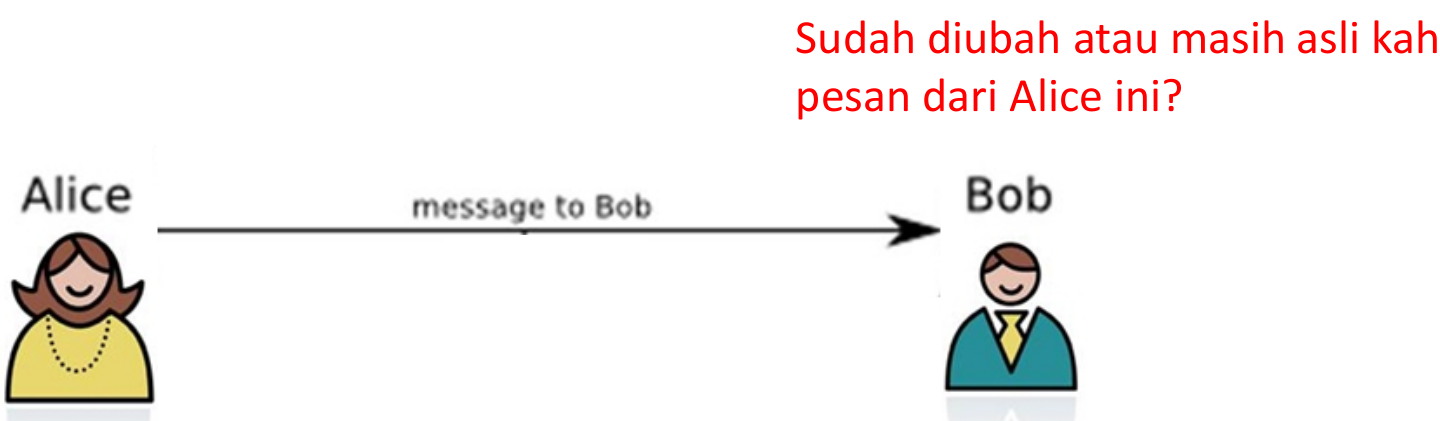
\includegraphics[width=157.50mm,height=115.83mm]{../../images/llm/page_008_img_01.png}%
\end{textblock*}

\end{document}
